\documentclass[10pt,twoside,czech,a4paper]{article}

\usepackage{polyglossia}
\setdefaultlanguage{czech}
\setotherlanguage{russian}

\usepackage{fontspec}
\defaultfontfeatures{Ligatures=TeX}
\setmainfont{Times New Roman}

\usepackage{graphicx}
\usepackage{url}
\usepackage{hyperref}
\usepackage{cite}
\usepackage{float}

\pagestyle{headings}

\title{P2P Protokoly pro přenos souborů\thanks{Semestrální projekt v předmětu Metody inženýrské práce, ak. rok 2023/24, vedení: Ing. Richard Marko, PhD.}}

\author{Andrei Yakuta\\[2pt]
	{\small Slovenská technická univerzita v Bratislavě}\\
	{\small Fakulta informatiky a informačních technologií}\\
	{\small \texttt{xyakuta@stuba.sk}}
	}


\begin{document}

\maketitle

\begin{abstract}
Tento článek se zabývá Peer-to-Peer (P2P) protokoly pro přenos souborů, které umožňují sdílení dat bez centrálního serveru.
P2P protokoly jako jsou BitTorrent, eDonkey a Gnutella, jsou zkoumány s ohledem na jejich architekturu, vyhledávání a sdílení souborů, a bezpečnostní opatření.
Dále článek porovnává P2P a tradiční client-server modely, hodnotí různé implementace P2P protokolů a diskutuje možný vývoj P2P technologií a jejich potenciální dopad na budoucí digitální aplikace a služby.
Závěrem poskytuje ucelený pohled na aktuální stav a perspektivy P2P technologií v oblasti přenosu souborů.
\end{abstract}



\section{Úvod}

P2P (Peer-to-Peer) protokoly pro přenos souborů představují způsob sdílení dat mezi uzly ve stejné síti bez nutnosti centrálního serveru.
Tento způsob sdílení dat umožňuje výrazné snížení nákladů na infrastrukturu, zatímco zajišťuje rychlý a spolehlivý přenos velkých souborů.
Protokoly Peer-to-Peer jsou v dnešní době velmi oblíbené, protože umožňují decentralizaci od serverů (což v dnešní době zabraňuje “zájemcům” mazat soubory, a tím podporuje svobodu slova).

V mém článku se zaměřím na analýzu různých P2P protokolů, jako jsou BitTorrent, eDonkey a Gnutella.
Hlavním cílem je porozumění architektuře těchto protokolů, mechanismům vyhledávání a sdílení souborů, a způsobům, jak tyto protokoly řeší problémy s bezpečností a soukromím.
Porovnám také P2P protokoly s tradičními client-server modely, abych diskutoval o výhodách a nevýhodách obou přístupů.
Důležitou součástí mé analýzy bude hodnocení různých implementací P2P protokolů a jejich dopad na výkon, škálovatelnost a odolnost proti chybám.
Dále se pokusím předvídat možný vývoj P2P technologií a zvážit jejich potenciální dopad na budoucí aplikace a služby v digitálním světě.


\section{Co je Peer-to-Peer?}

Pro počítačové systémy Peer-to-Peer (P2P) jsou charakteristická konsensuální spojení mezi "peery" (rovnocenní účastníci sítě).
To znamená, že počítače v síti mohou vzájemně komunikovat, aniž by měly procházet přes samostatný serverový počítač\cite{Bauwens2019}.
Z tohoto důvodu se při přechodu z Client-Server sítě na Peerto-Peer snižuje zatížení serveru, což je jedna z výhod používání protokolu P2P.
Navíc se zvyšuje rychlost přenosu dat a propustnost sítě.

Pokud jde o P2P síť, je charakteristické, že každý účastník sítě může plnit funkci serveru i klienta.
Při přenosu souborů prostřednictvím P2P protokolů to znamená, že každý účastník sítě, který stáhl část přenášeného souboru (funkce klienta), ji může předat ostatním účastníkům (funkce serveru).
Přitom se vůbec (nebo téměř vůbec) nepoužívá samostatný server.

Jednou z klíčových vlastností tohoto typu sítě pro přenos souborů je, že síť skoro není závislá na jediném serveru, tj. síť se nezhroutí, pokud ji někteří členové opustí, na rozdíl od sítě Client-Server, kde při výpadku serveru dojde k výpadku celé sítě.

Za zmínku stojí také to, že díky decentralizaci sítě P2P téměř není možné zastavit šíření jakýchkoli souborů v síti, protože všichni uživatelé v síti jsou servery.
Jinými slovy, na rozdíl od sítě Client-Server, kde by distribuce souborů skončila po vypnutí serveru, by museli být všichni členové sítě vyřazeni.


\section{P2P protokoly pro přenos souborů}

Ačkoli nejzákladnějším požadavkem na síť P2P je decentralizace od serveru, některé protokoly používají servery ke zjišťování informací o souborech nebo o uživatelích, od nichž lze určitý soubor převzít.
Na základě toho lze protokoly rozdělit do dvou různých skupin podle jejich architektury: čistá P2P a P2P zprostředkovaná serverem\cite{Lui2002}.

\subsection{Čisté P2P protokoly}

K této skupině patří protokoly jako Gnutella a Freenet.
Hlavní výhodou čistých P2P protokolů je, že síť, na rozdíl od P2P protokolů zprostředkovaných serverem, vůbec není závislá na serveru, protože žádný nemá.
Ale kvůli té nezávislosti musí dynamicky objevovat další partnery v síti, což způsobuje problémy, jako je vyšší spotřeba síťových prostředků a nízká škálovatelnost\cite{Lui2002}.

\begin{figure}[H]
	\centering
	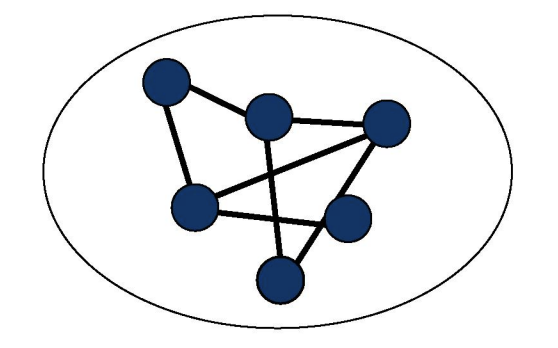
\includegraphics[width=0.5\textwidth]{pure-p2p.png}
	\caption{Architektura čisté P2P sítě. Zdroj \cite{Leong2007}}
	\label{fig:pure-p2p}
\end{figure}
	

\subsection{P2P protokoly zprostředkované serverem}

K této skupině patří protokoly jako eDonkey, Napster, a BitTorrent.
Jak bylo dříve zmíněno, jednou z nevýhod této skupiny P2P protokolů je, že síť je závislá na serveru.
I když se síť při výpadku serveru nezhroutí, P2P aplikace nebude schopna najít další peery\cite{Lui2002}.

\begin{figure}[H]
	\centering
	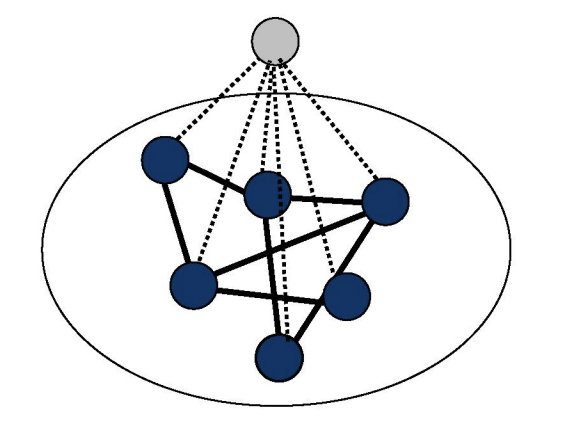
\includegraphics[width=0.5\textwidth]{server-mediated-p2p.png}
	\caption{Architektura P2P sítě zprostředkované serverem. Zdroj \cite{Leong2007}}
	\label{fig:server-mediated-p2p}
\end{figure}


\section{Srovnání P2P a tradičních client-server modelů}

P2P a tradiční client-server modely představují dva různé přístupy k organizaci a řízení síťové komunikace a sdílení dat.
Přestože mají oba modely své silné stránky a jsou vhodné pro různé účely, odlišují se v několika klíčových aspektech.

\begin{table}[H]
	\centering
	\begin{tabular}{|c|c|c|}
		\hline
		\textbf{Aspekt} & \textbf{P2P} & \textbf{Client-Server} \\
		\hline
		Decentralizace & Ano & Ne \\
		\hline
		Škálovatelnost & Vysoká & Omezená \\
		\hline
		Náklady & Rozložené & Centralizované \\
		\hline
		Bezpečnost & Variabilní & Vyšší \\
		\hline
		Rychlost & Vysoká & Závislá na serveru \\
		\hline
		Anonymita & Ano & Ne \\
		\hline
	\end{tabular}
	\caption{Srovnání P2P a client-server modelů}
\end{table}

\subsection{Decentralizace versus centralizace}

P2P model je charakterizován decentralizací, kde každý uzel (peer) v síti může fungovat jak jako klient, tak jako server, což podporuje distribuci dat a zajišťuje robustnost sítě při výpadku jednotlivých uzlů.
Na druhou stranu, client-server model je založen na centralizované architektuře, kde server poskytuje služby klientům a spravuje přístup k datům.
Výpadky serveru v client-server modelu mohou vést k výpadkům služby, zatímco v P2P modelu může síť nadále fungovat, dokud existuje dostatečný počet peerů.

\subsection{Škálovatelnost}

P2P sítě mají potenciál ke škálování, protože noví uživatelé mohou přispívat svými zdroji (např. bandwidth, úložným prostorem) k celkové kapacitě sítě.
Naopak, client-server modely mohou čelit omezením v škálovatelnosti, pokud server nedokáže zvládnout rostoucí počet klientů.

\subsection{Náklady na infrastrukturu}

V P2P modelu jsou náklady na infrastrukturu distribuovány mezi všechny učastníky sítě, což může vést k nižším celkovým nákladům ve srovnání s client-server modely, kde je potřeba investovat do silných a spolehlivých serverů, aby bylo možné zvládnout požadavky klientů \cite{Leibnitz2007}.

\subsection{Bezpečnost}

Client-server modely umožňují lepší kontrolu a správu dat a služeb, což může vést k vyšší úrovni bezpečnosti a spolehlivosti.
V P2P modelu může být obtížnější zajistit bezpečnost a integritu dat, zejména v otevřených P2P sítích, kde může dojít k většímu riziku neoprávněného přístupu a šíření škodlivého softwaru \cite{Leibnitz2007}.

Avšak v P2P sítích může decentralizovaná struktura ztížit vnějším pozorovatelům, jako jsou útočníci nebo autority, zjistit, kde jsou data uložena a kdo je sdílí, což může uživatelům poskytnout vyšší úroveň anonymity.
Naopak, v tradičních client-server modelůch je sledovatelnost jednodušší, protože veškerá komunikace prochází centrálním serverem, který může být snadno monitorován a analyzován.

\subsection{Rychlost a výkon}

Výkon a rychlost přenosu dat může být ve velkých P2P sítích výrazně vyšší, protože data mohou být přenášena paralelně od mnoha peerů.
Na druhou stranu, výkon client-server modelů může být omezen kapacitou serveru, zejména při vysoké zátěži.


\section{Hodnocení a dopad P2P protokolů}

\subsection{BitTorrent protokol}

BitTorrent je příkladem P2P sítě s centralizovanou strukturou (zprostředkovanou serverem).
Centrálním uzlem v této síti je tracker (server), který obsahuje informace o seznamu uzlů připojených k síti a službách poskytovaných jednotlivými uzly (např. seznam souborů dostupných ke stažení z daného uzlu).
Pro stažení požadovaného souboru uzel odesílá trackeru požadavek (pomocí HTTP protokolu) obsahující identifikátor požadovaného souboru, který se obvykle získává z torrent souboru (viz dále) \cite{Chokkalingam2004}.
Tracker odpovídá na tento požadavek seznamem uzlů, ve kterých je požadovaný soubor k dispozici\cite{Radchenko2012}.
Server nadále pomáhá uzlům vzájemně komunikovat, ačkoli poslední verze softwaru vyžadují server pouze v inicializační fázi (což umožňuje větší decentralizaci od serveru)\cite{Lande2008}.

Specifikem BitTorrentu je pojem torrent, který definuje relaci přenosu části souboru do množiny peerů.
Uživatel se obvykle připojí k existujícímu torrentu stažením .torrent souboru, který obsahuje metainformace o stahovaném souboru a IP adresu trackeru torrentu\cite{Legout2005, Chokkalingam2004}.

Podle protokolu BitTorrent se soubory přenášejí po částech, přičemž každý klient tyto části stahuje současně s tím, jak je předává ostatním klientům.
Tím se snižuje zatížení a závislost na každém zdrojovém klientovi\cite{Lande2008}.
Při dostatečně velkém počtu peerů se tím také výrazně zrychlí stahování souborů, což je velká výhoda tohoto protokolu při stahování velkých souborů\cite{Barakat2004}.

\begin{figure}[H]
	\centering
	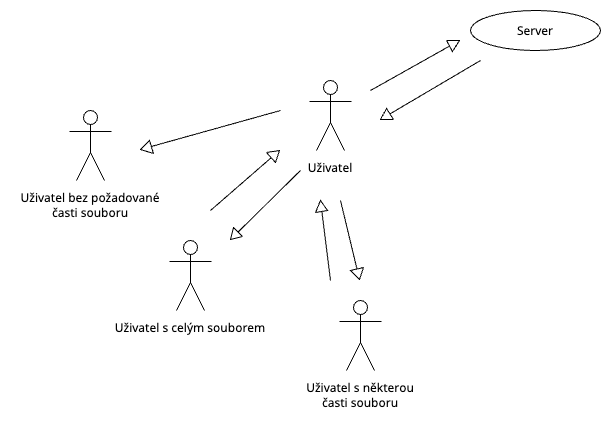
\includegraphics[width=0.75\textwidth]{BitTorrent.png}
	\caption{Architektura BitTorrent sítě}
\end{figure}

\subsection{Gnutella protokol}

Gnutella je příkladem P2P sítě s decentralizovanou strukturou (čisté P2P), která nevyžaduje centrální servery pro indexaci nebo vyhledávání souborů.
Na rozdíl od BitTorrentu, který využívá tracker pro koordinaci sdílení souborů, Gnutella funguje na plně decentralizovaném modelu.
Každý uzel v Gnutella síti může fungovat jak jako klient, tak jako server, což umožňuje přímé sdílení souborů mezi uživateli.
Tato architektura zajišťuje, že síť je odolnější proti výpadkům a obtížněji cenzurovatelná.

V Gnutella protokolu, když uživatel hledá soubor, jeho dotaz se přeposílá od uzlu k uzlu pomocí mechanismu zvaného "flooding".
Tento proces spočívá v rozesílání dotazu všem sousedním uzlům, které pak tento dotaz dále přeposílají, dokud není nalezen odpovídající soubor\cite{Howe2000}.
Skutečné stahování souboru porbíhá pomocí HTTP portokolu s uzlem, který první informoval, že soubor má \cite{Gnutella, Portmann2001}.
Ačkoliv tento způsob je efektivní pro nalezení souborů v malé síti, může způsobovat vysokou síťovou zátěž v rozsáhlejších sítích\cite{Ripeanu2001}.

Navzdory výzvám spojeným s decentralizací, jako jsou efektivita vyhledávání a bezpečnostní rizika, Gnutella představuje důležitý model v P2P technologiích.
Jeho přístup k distribuci a sdílení souborů zůstává významný pro svou schopnost podporovat svobodný a neomezený přenos informací mezi uživateli.
Avšak decentralizovaná povaha sítě ztěžuje implementaci bezpečnostních kontrol, a proto je Gnutella často vnímána jako méně bezpečná než jiné P2P sítě, jako je BitTorrent.

\begin{figure}[H]
	\centering
	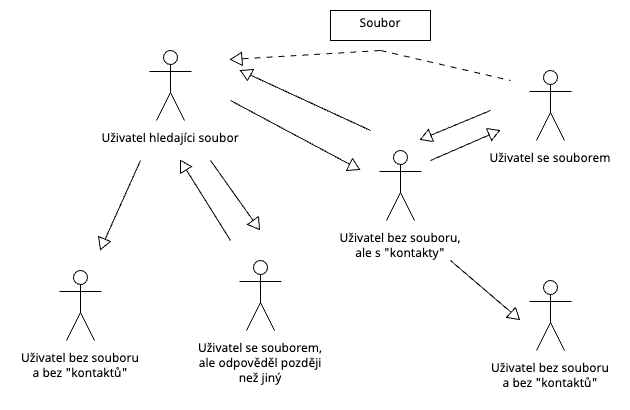
\includegraphics[width=0.75\textwidth]{Gnutella.png}
	\caption{Architektura Gnutella sítě}
\end{figure}


\section{Budoucnost P2P technologií}

S rostoucí digitalizací a vývojem technologií se očekává, že P2P technologie budou hrát klíčovou roli v budoucích inovacích.
Jedním z nejperspektivnějších směrů je vývoj nových protokolů, které spojují výhody P2P a tradičních client-server modelů.
Tyto hybridní protokoly by mohly nabídnout vyšší efektivitu, lepší škálovatelnost a větší bezpečnost.

P2P sítě by tak mohly být lépe integrovány do cloudových služeb, což by umožnilo lepší správu a distribuci dat.
Kromě toho se očekává, že P2P technologie budou hrát významnou roli v oblastech jako decentralizované úložiště dat, správa velkých dat a vývoj decentralizovaných aplikací (DApps), které jsou stále více populární v blockchainovém prostředí.
Tyto inovace by mohly výrazně ovlivnit způsob, jakým lidé sdílejí a spravují digitální obsah, a otevřít cestu pro nové formy digitální interakce a kolaborace.\cite{Kisembe2017}


\section{Rozšířené pohledy na P2P technologie}

\paragraph{Společenské souvislosti.}

Společenské souvislosti informatiky jsou neoddělitelné od jejího vývoje a aplikace.
P2P technologie, jako klíčový příklad, ukazují, jak informatika přispívá k decentralizaci informací a demokratizaci přístupu.
Tento model sdílení zásadně ovlivňuje, jak lidé komunikují, sdílejí obsah a spolupracují.
Je to zřetelné například v oblastech jako jsou sociální média, kde P2P mechanismy umožňují uživatelům přímou výměnu informací a názorů, čímž se rozšiřují možnosti pro kolektivní akci a společenské hnutí.
P2P také významně ovlivňuje průmysl, jako jsou média a zábava, kde umožňuje nové formy distribuce obsahu, což mění tradiční paradigma vlastnictví a přístupu k digitálním zdrojům.

\paragraph{Historické souvislosti.}

Historie informatiky je historií inovací a revolucí. P2P protokoly, jako je BitTorrent, představují významný milník v této historii, jelikož představují odchod od centralizovaných modelů datového sdílení.
Vznik P2P v raných 2000. letech signalizoval novou éru v síťových technologiích, která umožnila rozšíření velkých souborů bez potřeby masivních serverových zdrojů.
Tento posun přinesl zásadní změny v přístupu k digitálnímu obsahu a otevřel cestu pro další inovace, jako jsou decentralizované aplikace a blockchain technologie.
Historie informatiky je tedy příběhem postupného přesunu od centralizované k decentralizované kontrole, což odráží širší společenské změny v pojetí informací a technologie.

\paragraph{Technologie a lidé.}

Vztah mezi technologií a lidmi je v informatice klíčový.
P2P protokoly demonstrují, jak technologie mohou posílit individuální uživatele tím, že jim dávají větší kontrolu nad způsobem, jakým přistupují a sdílejí informace.
Například, decentralizované sítě poskytují uživatelům větší ochranu soukromí a snižují závislost na centrálních autoritách.
Tento přístup k technologii vede k větší autonomii uživatelů a podporuje myšlenku, že technologie by měly sloužit lidem, a ne naopak.
P2P technologie také otevírají nové možnosti pro spolupráci a inovace, protože umožňují lidem sdílet zdroje a znalosti efektivněji a na globální úrovni.

\paragraph{Udržitelnost a etika.}

Udržitelnost a etika v informatice jsou nezbytné pro zajištění, že technologický rozvoj probíhá způsobem, který je ohleduplný k životnímu prostředí a etickým normám.
P2P technologie mohou přispět k udržitelnosti tím, že snižují potřebu fyzických serverů a infrastruktury, což vede k nižší spotřebě energie a lepšímu využití zdrojů.
Z etického hlediska P2P podporuje principy jako jsou svoboda projevu a rovný přístup k informacím.
Nicméně, vyvstávají etické otázky ohledně autorských práv a distribuce chráněného obsahu.
Je tedy nezbytné, aby vývojáři a uživatelé P2P technologií pečlivě zvažovali etické důsledky svých akcí a usilovali o vyvážený přístup, který respektuje práva jednotlivců a společnosti jako celku.


\section{Závěr}

V tomto článku byla prozkoumána dynamika a vliv Peer-to-Peer protokolů v kontextu současného digitálního světa.
Porovnáním s tradičními client-server modely jsou odhalené jedinečné výhody P2P přístupu, zejména v decentralizaci, škálovatelnosti a efektivitě přenosu dat.
Prostřednictvím případových studií protokolů jako BitTorrent a Gnutella je ukázáno, jak různé P2P systémy přistupují k přenosu souborů a jak řeší výzvy, jako jsou bezpečnost, vyhledávání a distribuce dat.

Význam P2P technologií se neustále zvyšuje v době, kdy digitalizace a požadavky na ukládání dat rychle rostou.
Vzhledem k jejich potenciálu pro rozvoj decentralizovaných aplikací a integraci s blockchainovými technologiemi, se očekává, že P2P protokoly budou hrát klíčovou roli v budoucích technologických inovacích.
Budoucnost P2P technologií může zahrnovat nové hybridní protokoly, které kombinují nejlepší aspekty P2P a client-server modelů, čímž poskytnou silnější, bezpečnější a efektivnější systémy pro sdílení a správu digitálního obsahu.

Závěrem lze říci, že P2P technologie nejenže představují významnou část současného digitálního ekosystému, ale budou také hrát zásadní roli v jeho budoucím vývoji.
Ať už jde o podporu svobody projevu, efektivní distribuci dat, nebo podporu nových inovací, P2P protokoly jsou klíčovým prvkem pro budoucí digitální krajinu.


\bibliography{literatura}
\bibliographystyle{abbrv}
\end{document}
